\documentclass[12pt, a4paper]{article}

\usepackage{amsmath}
\usepackage{array}
\usepackage{amsmath}
\usepackage[portuguese]{babel}
\usepackage{chngpage}
\usepackage{float}
\usepackage[a4paper, margin=2cm]{geometry}
\usepackage{graphicx}
\usepackage{hyperref}
\usepackage{setspace}
\usepackage{xcolor}

\title{\Huge \textbf{Computação Gráfica \\ \Large Trabalho Prático -- Fase I}}
\date{2 de março 2025}
\author{Grupo 3}

\begin{document}

\begin{center}
    
\includegraphics[width=0.25\textwidth]{res/cover/EE-C.eps}
\end{center}

\chardef\_=`_
\onehalfspacing
\setlength{\parskip}{\baselineskip}
\setlength{\parindent}{0pt}
\def\arraystretch{1.5}

{\let\newpage\relax\maketitle}
\maketitle
\thispagestyle{empty}

\vspace*{\fill}

\begin{adjustwidth}{-2cm}{-2cm} % These values only need to be large enough to center the table
    \begin{center}
        \begin{tabular}{>{\centering}p{0.25\textwidth}
                        >{\centering}p{0.25\textwidth}
                        >{\centering}p{0.25\textwidth}
                        >{\centering\arraybackslash}p{0.25\textwidth}}
            
\includegraphics[width=3.5cm]{res/cover/A104437.png} &
            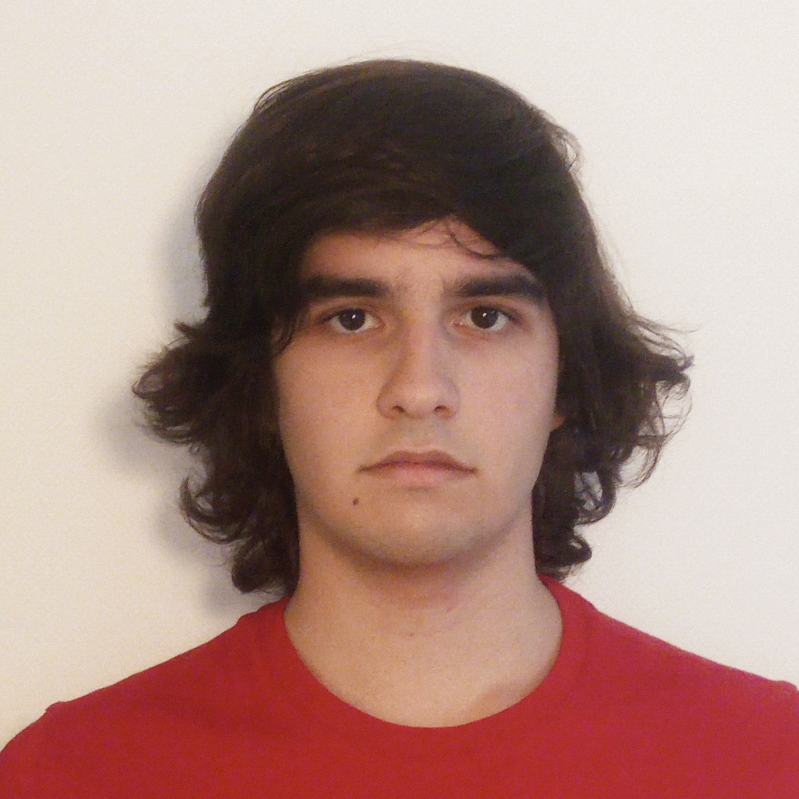
\includegraphics[width=3.5cm]{res/cover/A104348.png} &
            
\includegraphics[width=3.5cm]{res/cover/A90817.png} &
            
\includegraphics[width=3.5cm]{res/cover/A104179.png} \\

            Ana Oliveira & Humberto Gomes & Mariana Cristino & Sara Lopes \\
            A104437      & A104348        & A90817           & A104179
        \end{tabular}
    \end{center}
\end{adjustwidth}

\pagebreak

\begin{abstract}
    \textbf{\color{red} TODO - resumo}
\end{abstract}

\section{\emph{Generator}}

\subsection{Descrição e uso}

\textbf{\color{red} TODO - descrição e uso do programa}

\subsection{Formato \texttt{.3d}}

Visto que a estrutura de um ficheiro \texttt{.3d} separa os vértices de um modelo das suas faces, o
processo de criação dos modelos 3D dos vários sólidos é dividido em duas fases: a geração do
conjunto de pontos que os constituem, e o seu agrupamento em faces triangulares.

\subsection{Plano}

O primeiro passo para a geração da nuvem de pontos de um plano é o cálculo do comprimento de uma
divisão, $d = \frac{L}{N}$, onde $L$ simboliza o comprimento do plano e $N$ o número de divisões.
Depois, determinam-se os dois vetores que definem a direção do plano. Estes poderiam ser os vetores
diretores dos eixos $x$ e $z$, mas é mais simples que estes tenham o comprimento de uma divisão do
plano.

$$
\vec{\imath} = (d, 0, 0)
\hspace{1cm}
\vec{\jmath} = (0, 0, d)
$$

Depois, encontra-se o ponto do plano com os menores valores das coordenadas $x$ e $z$. Como se
deseja que o plano esteja centrado na origem, as coordenadas $x$ e $z$ do ponto desejado serão o
simétrico da metade do comprimento do plano:

$$
P_0 = \left ( - \frac{L}{2}, 0, - \frac{L}{2} \right )
$$

Depois, qualquer ponto $P$ do plano pode ser definido como a adição a $P_0$ de uma combinação linear
de $\vec{\imath}$ e $\vec{\jmath}$, limitando a números inteiros os coeficientes multiplicativos dos
vetores:

$$
P = P_0 + \alpha \, \vec{\imath} + \beta \, \vec{\jmath}
\hspace{1cm}
\alpha, \beta \in \left \lbrace 0, 1, \ldots, N \right \rbrace
$$

Na prática, o plano é gerado iterando pelos valores inteiros possíveis de $\alpha$ e de $\beta$,
incrementando primeiro $\beta$, e só depois de $\alpha$, o que dá origem a uma nuvem de pontos como
a que pode ser observada na figura abaixo:

\begin{figure}[H]
    \centering
    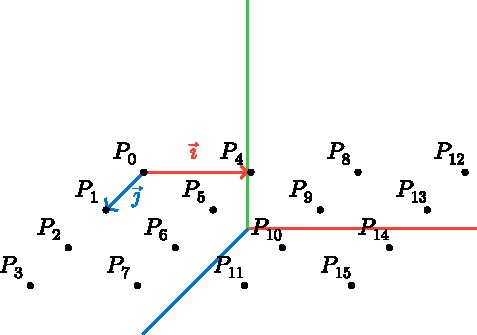
\includegraphics[width=0.4\textwidth]{res/figures/PlanePoints.pdf}
    \caption{Nuvem de pontos resultante da geração de um plano de três divisões.}
\end{figure}

Depois, os vértices gerados podem ser agrupados nos triângulos que formam o plano. Para tal,
começa-se com o primeiro vértice do plano, $P_0$. Considera-se também o vértice seguinte, $P_1$, e
os dois vértices com os valores de $z$ de $P_0$ e $P_1$, mas com o seguinte valor de $x$ possível
(na "linha"{} seguinte). Um exemplo de um conjunto destes quatro vértices pode ser visto na figura
abaixo. Com estes vértices, gera-se um quadrado, ou seja, dois triângulos. Este processo repete-se
para todos os vértices onde é aplicável, ou seja, todos com exceção dos pontos com os maiores
valores de $x$ ou de $z$ possíveis.

\begin{figure}[H]
    \centering
    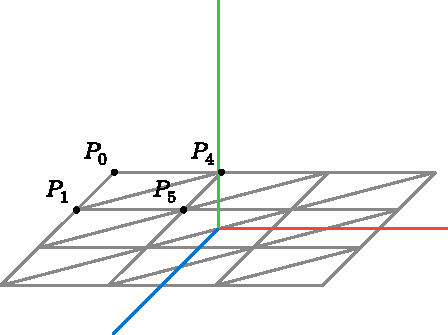
\includegraphics[width=0.4\textwidth]{res/figures/PlaneTriangles.pdf}
    \caption{
        Triângulos de um plano gerado, e pontos utilizados na primeira iteração do ciclo de geração
        de triângulos.
    }
\end{figure}

Uma otimização feita pela \emph{engine} é \emph{face culling}, ou seja, desenhar apenas as faces
voltadas para a câmara. No caso do plano, deseja-se que os seus triângulos estejam voltados para
cima, pelo que os seus vértices devem estar ordenados na ordem contrária à dos ponteiros do
relógio. Para os quatro pontos apresentados acima, os triângulos gerados são os seguintes:

$$
T_1 = (P_1, P_4, P_0)
\hspace{1cm}
T_2 = (P_1, P_5, P_4)
$$

\subsection{Cubo}

De um modo simples, o processo de geração de um cubo consiste na repetição da geração de um plano
seis vezes, uma vez para cada face. No entanto, algumas diferenças devem ser evidenciadas. Tal como
no plano, após ser calculado o comprimento de uma divisão do cubo, são definidos os vetores
diretores dos vários planos que são as faces do cubo. Há três pares de vetores diretores, cada um
utilizado para gerar duas faces opostas:

$$
\begin{array}{ll>{\hspace{1cm}}ll>{\hspace{1cm}}c}
    \vec{\imath_1} &= (1, 0, 0) &
    \vec{\jmath_1} &= (0, 1, 0) &
    (\text{faces dianteira e traseira}) \\
    \vec{\imath_2} &= (0, 1, 0) &
    \vec{\jmath_2} &= (0, 0, 1) &
    (\text{faces esquerda e direita}) \\
    \vec{\imath_3} &= (0, 0, 1) &
    \vec{\jmath_3} &= (1, 0, 0) &
    (\text{faces superior e inferior})
\end{array}
$$

Ao contrário do que acontece no plano, estes vetores encontram-se normalizados, o que é útil para
determinar o ponto de cada face a partir do qual os seus restantes pontos serão gerados. Tal como
acontece no plano, para o cubo estar centrado na origem, é necessário que todas as coordenadas deste
ponto inicial estejam a uma distância de $\frac{L}{2}$ da origem, onde $L$ representa o comprimento
do lado do cubo. Por exemplo, para o primeiro par de vetores diretores, os pontos são os seguintes,
correspondentes às faces traseira e dianteira, respetivamente:

$$
P_{0^-} = \left ( -\frac{L}{2}, -\frac{L}{2}, -\frac{L}{2} \right )
\hspace{1cm}
P_{0^+} = \left ( -\frac{L}{2}, -\frac{L}{2}, +\frac{L}{2} \right )
$$

De um modo geral, nas coordenadas onde $\vec{\imath}$ ou $\vec{\jmath}$ têm um valor não nulo, a
coordenada do ponto inicial é $-\frac{L}{2}$. A coordenada restante pode assumir, conforme a face,
ou $\frac{L}{2}$ ou $-\frac{L}{2}$. Matematicamente, o vetor perpendicular à face é dado por:

$$
\vec{n} = (1, 1, 1) - \vec{\imath} - \vec{\jmath}
$$

A partir deste vetor, os pontos iniciais das faces são dados por:

$$
P_{0^-} = -\frac{L}{2} \left ( \vec{\imath} + \vec{\jmath} + \vec{n} \right )
\hspace{1cm}
P_{0^+} = -\frac{L}{2} \left ( \vec{\imath} + \vec{\jmath} - \vec{n} \right )
$$

Com os vetores diretores e os pontos iniciais de cada face, é possível normalizar os vetores
diretores e gerar os pontos de cada face, seguindo o mesmo processo utilizado para o plano. Abaixo,
apresenta-se um exemplo da nuvem de pontos de um cubo gerado:

\begin{figure}[H]
    \centering
    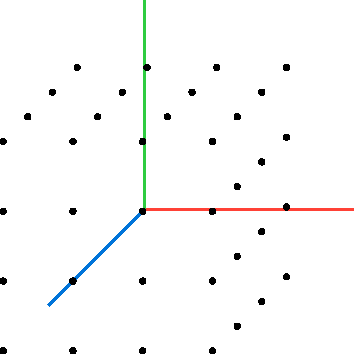
\includegraphics[width=0.35\textwidth]{res/figures/CubePoints.pdf}
    \caption{
        \onehalfspacing
        Nuvem de pontos resultante da geração de um cubo de três divisões. Os pontos das faces
        ocultas não foram representados nesta figura.
    }
\end{figure}

Depois de gerada a nuvem de pontos, o processo de geração dos triângulos de cada face é muito
semelhante ao do plano. No entanto, a ordem dos vértices de cada triângulo difere conforme a face do
cubo a ser construída. Considere-se o exemplo abaixo, o das faces superior e inferior de um cubo com
apenas uma divisão:

\begin{figure}[H]
    \centering
    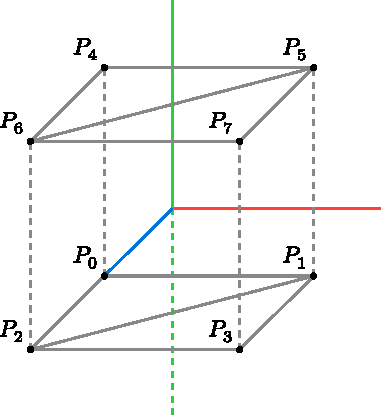
\includegraphics[width=0.35\textwidth]{res/figures/CubeFaces.pdf}
    \caption{Faces superior e inferior de um cubo de apenas uma divisão.}
\end{figure}

Para que os triângulos da face inferior estejam voltados para o exterior do cubo, ou seja, para
baixo, os seus pontos são ordenados no sentido dos ponteiros do relógio:

$$
T_1 = (P_1, P_2, P_0)
\hspace{1cm}
T_2 = (P_1, P_3, P_2)
$$

Na face superior, a ordem dos pontos dos triângulos é contrária, no sentido contrário ao dos
ponteiros do relógio:

$$
T_1' = (P_5, P_4, P_6)
\hspace{1cm}
T_2' = (P_7, P_5, P_6)
$$

Para cada par de faces opostas, cada face será sujeita, conforme o seu vetor normal, a uma ordenação
distinta dos pontos dos seus triângulos. Após aplicar o processo de geração de triângulos a todas as
faces, é dada por concluída a construção do modelo do cubo.

\begin{figure}[H]
    \centering
    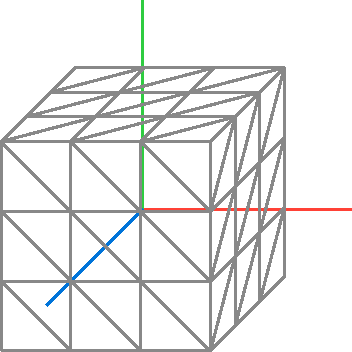
\includegraphics[width=0.35\textwidth]{res/figures/CubeTriangles.pdf}
    \caption{
        \onehalfspacing
        Triângulos resultantes da geração de um cubo de três divisões. As faces ocultas não foram
        representadas nesta figura.
    }
\end{figure}

\subsection{Esfera}

Para a construção da esfera, utilizámos um sistema de coordenadas esféricas,
no qual a posição de cada ponto na esfera é determinada por dois ângulos: o
ângulo polar \( \theta \) e o ângulo azimutal \( \phi \).

A parametrização de um ponto sobre uma esfera de raio \( r \) pode ser definida pelas seguintes
equações:
\[
x = r \sin(\theta) \cos(\phi)
\]
\[
y = r \cos(\theta)
\]
\[
z = r \sin(\theta) \sin(\phi)
\]
onde:
\begin{itemize}
\item \( \theta \) é o ângulo polar, que varia entre \( 0 \) (pólo norte) e \( \pi \)
(pólo sul), que determina a latitude do ponto na esfera;
\item \( \phi \) é o ângulo azimutal que varia entre \( 0 \) e \( 2\pi \), que define a
longitude do ponto.
\end{itemize}

Este modelo matemático permite gerar uma esfera distribuída no espaço tridimensional.
No entanto, para a sua implementação computacional, é necessário discretizar estes valores e
definir um conjunto finito de pontos e faces que aproximem à sua forma contínua.

\subsubsection{Geração dos Vértices}
Para discretizar a superfície da esfera, divide-se o intervalo de \( \theta \) em stacks
(fatias horizontais) e o intervalo de \( \phi \) em slices (segmentos verticais). Assim,
as incrementações angulares são calculados da seguinte forma:
\[
\Delta\theta = \frac{\pi}{\text{stacks}}, \quad \Delta\phi = \frac{2\pi}{\text{slices}}
\]
Ao percorrer os valores de \( \theta \) e \( \phi \), é possível gerar um conjunto ordenado
de pontos distribuídos sobre a esfera.

De modo que, a construção dos vértices segue os seguintes passos:

1. Criação do pólo norte: O primeiro ponto criado é o pólo norte, localizado em
\( (0, r, 0) \).

2. Geração dos Pontos Intermédios: Para cada stack (exceto as extremidades, que
são os pólos), iterámos sobre os valores de \( \theta \), determinámos a altura \( y \) do ponto
e o raio da secção circular correspondente:
\[
y = r \cos(\theta)
\]
\[
r_{\text{secção}} = r \sin(\theta)
\]
Para cada slice, iterámos sobre os valores de \( \phi \), é calculada a posição dos pontos
na secção circular:
\[
x = r_{\text{secção}} \cos(\phi)
\]
\[
z = r_{\text{secção}} \sin(\phi)
\]

3. Criação do pólo sul: Após a geração das stacks intermédias, é criado o pólo sul
em \( (0, -r, 0) \).

\subsubsection{Construção das Faces}
Após a geração dos vértices, é necessário definir as faces triangulares que compõem a superfície
esférica. A triangulação é realizada da seguinte forma:

1. Ligação ao pólo norte: Cada ponto da primeira stack (exceto o pólo norte) forma um
triângulo com o pólo norte e o ponto seguinte na mesma stack. Para garantir a continuidade circular,
o último ponto da stack liga-se novamente ao primeiro, ou seja, os vértices são ligados de forma a
criar uma face triangular:
\[
T_1 = (P_1, P_3, P_2)
\]

\begin{figure}[H]
    \centering
    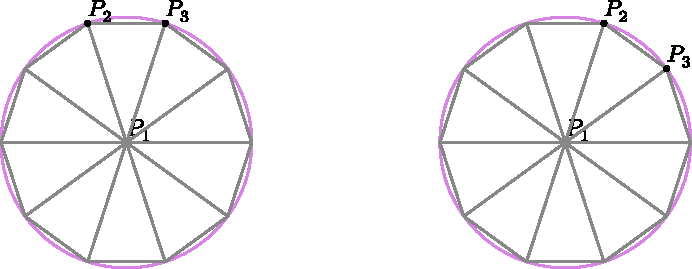
\includegraphics[width=0.4\textwidth]{res/figures/polosSphere.pdf}
    \caption{
        Ilustração da ligação dos vértices da primeira stack ao pólo norte, formando os triângulos
        iniciais da esfera e a seguinte iteração.
    }
\end{figure}

2. Ligação das stacks intermédias:
Para cada fatia horizontal da esfera, os vértices são ligados de forma a criar duas faces
triangulares por quadrilátero:
\[
T_1 = (P_1, P_3, P_4)
\]
\[
T_2 = (P_1, P_4, P_2)
\]

\begin{figure}[H]
    \centering
    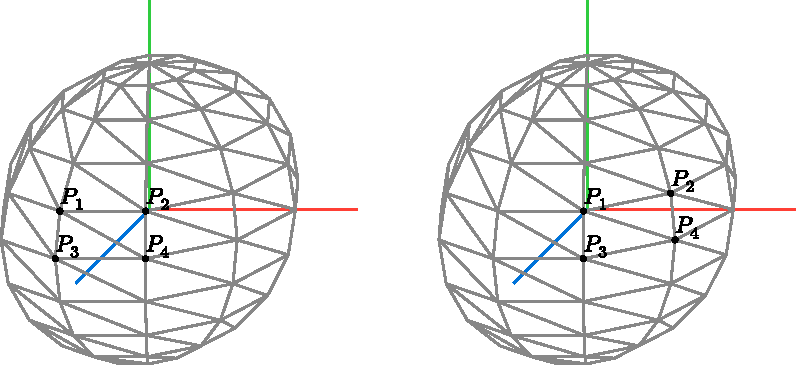
\includegraphics[width=0.4\textwidth]{res/figures/sphere.pdf}
    \caption{
        Triângulos de uma esfera gerada, e os pontos utilizados numa iteração do ciclo de geração
        de triângulos e na seguinte.
    }
\end{figure}

Este método assegura uma ligação contínua entre os pontos e evita a repetição de vértices
desnecessários.

3. Ligação ao pólo sul: O mesmo processo utilizado para o pólo norte é aplicado à stack
mais próxima do pólo sul, assim, garante que todas as fatias inferiores são corretamente ligadas ao
vértice final.
No entanto, a ordem dos vértices nos triângulos é invertida em comparação com o pólo norte.
Esta inversão garante que a normal de cada triângulo aponta para baixo, conforme ilustrado nos
círculos da primeira figura. No pólo norte, os vértices são ordenados no sentido anti-horário
(por exemplo, $P_1$, $P_3$, $P_2$), enquanto que no pólo sul, a ordem é invertida
($P_1$, $P_2$, $P_3$).

Este método proporciona uma representação eficiente e visualmente precisa, garante uma
boa distribuição das faces ao longo da sua superfície.

\subsection{Cilindro}

Para a construção do cilindro, utilizámos um sistema de coordenadas cilíndricas, onde a
posição de cada ponto é determinada pelo raio, pelo ângulo azimutal \( \phi \) e
pela altura \( y \).

A parametrização de um vértice sobre um cilindro de raio \( r \) e altura \( h \) pode ser definida
pelas seguintes equações:
\[
x = r \cos(\phi)
\]
\[
y = h
\]
\[
z = r \sin(\phi)
\]
onde:
\begin{itemize}
\item \( \phi \) é o ângulo azimutal, varia entre \( 0 \) e \( 2\pi \), que determina a
posição do ponto ao longo da circunferência da base.
\item \( y \) representa a altura, varia entre \( 0 \) (base inferior) e \( h \)
(base superior).
\end{itemize}

Este modelo matemático permite representar um cilindro tridimensionalmente. Para a sua implementação
computacional, discretizamos estes valores, onde é gerado um conjunto finito de pontos e faces que
aproximam à sua forma contínua.

\subsubsection{Geração dos Vértices}
Para discretizar a superfície do cilindro, o intervalo de \( \phi \) é dividido em slices
(segmentos verticais), enquanto a altura \( y \) é dividida em stacks (fatias horizontais).
Assim, os incrementos são calculados da seguinte forma:
\[
\Delta \phi = \frac{2\pi}{\text{slices}}, \quad \Delta y = \frac{h}{\text{stacks}}
\]

Os vértices são gerados da seguinte forma:

1. Criação da superfície lateral: Para cada stack ao longo da altura, iterámos
sobre os valores de \( \phi \), determinando a posição dos pontos na circunferência da secção
correspondente.

2. Criação dos vértices centrais das bases: Após gerar os pontos da superfície lateral,
adicionamos dois vértices centrais:
\begin{itemize}
\item O centro da base superior, localizado em \( (0, h, 0) \).
\item O centro da base inferior, localizado em \( (0, 0, 0) \).
\end{itemize}

\subsubsection{Construção das Faces}
Após a geração dos vértices, definimos as faces triangulares que compõem o cilindro. Esta etapa
é realizada em três partes:

1. Construção da superfície lateral:
Cada quadrilátero entre duas stacks sucessivas é dividido em duas faces triangulares:
\[
T_1 = (P_4, P_6, P_7)
\]
\[
T_2 = (P_4, P_7, P_5)
\]
Isto garante uma cobertura uniforme da superfície do cilindro.

\begin{figure}[H]
    \centering
    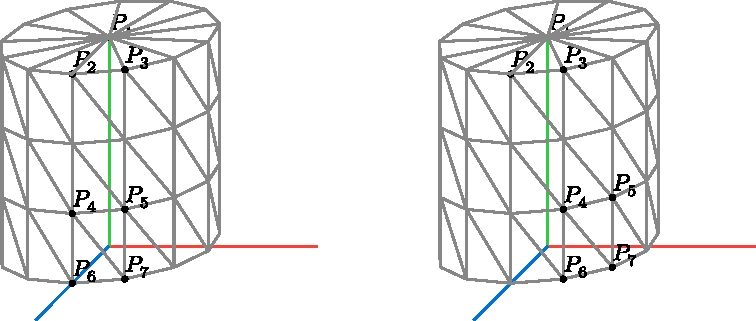
\includegraphics[width=0.4\textwidth]{res/figures/cylinder.pdf}
    \caption{
        Triângulos de uma esfera gerada, e os pontos utilizados numa iteração do ciclo de geração
        de triângulos e na seguinte.
    }
\end{figure}

2. Construção da base superior:
Cada ponto da última stack é ligado ao vértice central da base superior, de modo a formar
triângulos radiais:
\[
T = (P_1, P_2, P_3)
\]

3. Construção da base inferior:
O mesmo processo é repetido para a base inferior, o que garante o desenho correto da estrutura.

A ordem dos vértices cumpre a regra da orientação anti-horária, onde a correta
aplicação da técnica de face culling cumpre-se, que otimiza o processo de renderização
ao eliminar automaticamente as faces voltadas para trás.

Este método resulta numa representação eficiente e precisa do cilindro, mantendo uma boa
distribuição das faces sobre a sua superfície.

\section{\emph{Engine}}

\textbf{\color{red} TODO - \emph{engine}}

\section{Resultados obtidos}

\textbf{\color{red} TODO - resultados}

\section{Conclusão e Trabalho Futuro}

A primeira fase do projeto foi concluída com sucesso, de modo que os objetivos previamente definidos
foram alcançados. A implementação de Vertex Buffer Objects (VBOs) para a otimização da renderização
representa um avanço significativo na eficiência do engine, permitindo um processamento mais rápido
e eficaz dos dados dos vértices.

Em relação ao trabalho futuro, pretendemos realizar uma reestruturação da organização hierárquica do
mundo. A abordagem inicial, que privilegiava uma estrutura linear, será substituída por um sistema
de grupos que permitirá a aplicação de transformações a conjuntos de modelos de forma simultânea.
Esta alteração, motivada pela análise das fases subsequentes do projeto, possibilitará a gestão
eficiente de objetos relacionados.

Adicionalmente, tencionámos expandir as capacidades da câmara, implementando três modos distintos de
visualização: orbital, livre e em terceira pessoa. Esta diversidade de perspetivas enriquecerá a
experiência do utilizador e permitirá a exploração de diferentes estilos de interação com as cenas
3D.

A implementação das transformações geométricas solicitadas na segunda fase – translação, rotação e
escala – é um objetivo prioritário. Estas funcionalidades são essenciais para uma manipulação
precisa dos objetos na cena.

Acreditámos que estas melhorias e adições consolidarão o engine como uma ferramenta robusta e
versátil para a criação de mundos 3D.

\begingroup
\section{Bibliografia}
\renewcommand{\section}[2]{}

\begin{thebibliography}{9}
    \bibitem{exemplo}
        \href{https://youtu.be/dQw4w9WgXcQ}{Um item de exemplo na bibliografia}
    \bibitem{esfera}
        "OpenGL Sphere."{} Songho CA. Accessed: Mar. 1, 2025. [Online.] Available:
        \url{https://www.songho.ca/opengl/gl_sphere.html}
    \bibitem{cilindro}
        "OpenGL Cylinder, Prism \& Pipe."{} Songho CA. Accessed: Mar. 1, 2025. [Online.] Available:
        \url{https://www.songho.ca/opengl/gl_cylinder.html}
\end{thebibliography}
\endgroup

\end{document}
